\chapter{Marketing Analytics}

\begin{remark}{Outline}
In this chapter, we present two different marketing real-world example-dependent 
cost-sensitive problems, namely, churn modeling and direct marketing. Both problems deal 
with identifying those customers with certain characteristic with the objective to maximize the 
results of the different CRM strategies.
First, we introduce the churn modeling problem in Section \ref{sec:4:churn}. Lastly in Section 
\ref{sec:4:directmarketing}, the direct marketing problem is presented.
\end{remark}


\section{Churn modeling}
\label{sec:4:churn}

Customer churn predictive modeling deals with predicting the probability of a customer defecting 
using historical, behavioral and socio-economical information. This tool is of great benefit to 
subscription based companies allowing them to maximize the results of retention campaigns. The 
problem of churn predictive modeling has been widely studied by the data mining and machine learning
communities. It is usually tackled by using classification algorithms in order to learn the 
different patterns of both the churners and non-churners. Nevertheless, current state-of-the-art 
classification algorithms are not well aligned with commercial goals, in the sense that, the models 
miss to include the real financial costs and benefits during the training and evaluation phases. In 
the case of churn, evaluating a model based on a traditional measure such as accuracy or predictive 
power, does not yield to the best results when measured by the actual financial cost, ie. 
investment per subscriber on a loyalty campaign and the financial impact of failing to detect a 
real churner versus wrongly predicting a non-churner as a churner.

In this section, we present a cost-sensitive framework for customer churn predictive modeling, 
that we proposed in \citep{CorreaBahnsen2015a}. First, in Section \ref{sec:4:1:intro}, we introduce 
the problem of chrun modeling. Then in Section \ref{sec:4:1:evaluation}, we present a financial 
based measure for evaluating the effectiveness of a churn campaign taking into account the available 
portfolio of offers, their individual financial cost and probability of offer acceptance depending 
on the customer profile. Finally, in Section \ref{sec:4:1:data}, we describe the real-world churn 
modeling dataset that will be used during the experiments.


\subsection{Introduction to Churn Modeling}
\label{sec:4:1:intro}

The two main objectives of subscription-based companies are to  acquire new subscribers and 
retain those they already have, mainly because profits are directly linked with the number of 
subscribers.  In order to maximize the profit, companies must increase the customer base by 
incrementing sales  while decreasing the number of churners. Furthermore, it is common knowledge 
that retaining a  customer is about five times less expensive than acquiring a new one 
\citep{Farris2010}, this creates  pressure to have better and more effective churn campaigns.

A typical churn campaign consists in identifying from the current customer base which ones are 
more likely to leave the company, and make an offer in order to avoid that behavior.
With this in mind the companies use intelligence to create and improve retention and collection
strategies. In the first case, this usually implies an offer that can be either a discount or a 
free upgrade during certain span of time. In both cases the company has to 	assume a cost for that 
offer, therefore, accurate prediction of the churners becomes important. The logic of this flow is 
shown in \figurename{ \ref{fig:ch4:1}}.

	\begin{figure}[htbp]
	  \centering
    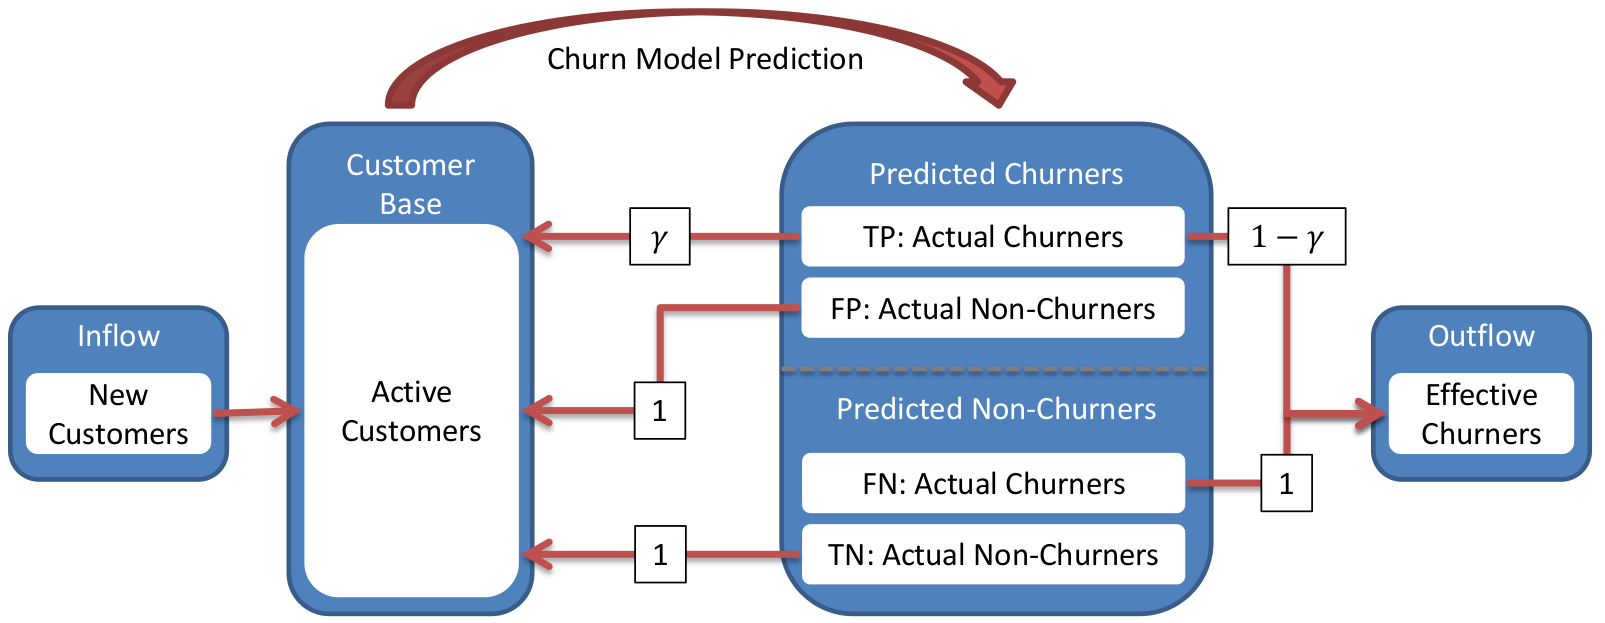
\includegraphics[width=11.5cm]{ch4_fig1}   %CHANGE TO 12cm
	  \caption{Flow analysis of a churn campaign \citep{Verbraken2012}}
	  \label{fig:ch4:1}
	\end{figure}

\begin{remark}{Flow analysis of a churn campaign}
The typical churn campaign process starts with the sales that every month increase the customer 
base, however, monthly there is a group of customers that decide to leave the company for many 
reasons. Then the objective of a churn model is to identify those customers before they take the 
decision of defecting.

Using a churn model, those customers more likely to leave are predicted as churners and 
an offer is made in order to retain them. However, it is known that not all customers will accept 
the offer, in the case when a customer is planning to defect, it is possible that the offer is not 
good enough to retain him or that the reason for defecting can not be influenced by an offer.
Using historical information, it is estimated that a customer will accept the offer with 
probability $\gamma$.
On the other hand, there is the case in which the churn model misclassified a non-churner as 
churner, also known as false positives, in that case the customer will always accept the offer that 
means and additional cost to the company since those misclassified customers do not have the 
intentions of leaving.

In the case were the churn model predicts customers as non-churners, there is also the possibility 
of a misclassification, in this case an actual churner is predicted as non-churner, since 
these customers do not receive an offer and they will leave the company, these cases are known as 
false negatives. Lastly, there is the case were the customers are actually non-churners, then 
there is no need to make a retention offer to these customers since they will continue to be part 
of the customer base.
\end{remark}

It can be seen that a churn campaign (or churn model) have three main points. First, avoid false 
positives since there is a financial cost of making an offer were it is not needed. Second, to the 
true positives, give the right offer that maximize $\gamma$ while maximizing the profit of the 
company. And lastly, to decrease the number of false negatives.

From a machine learning perspective, a churn model is a classification algorithm.
In the sense that using historical information, a prediction of which current customers 
are more likely to defect, is made. This model is normally created using one of a number of 
well establish algorithms (Logistic regression, neural networks, random forests, among 
others) \citep{Ngai2009,KhakAbi2010}. Then, the model is evaluated using measures such as 
misclassification error, receiver operating characteristic ($ROC$),  Kolmogorov-Smirnov ($KS$) 
or \mbox{$F_1Score$} statistics \citep{Verbeke2012}. However these measures assume that 
misclassification errors     carry the same cost, which is not the case in churn modeling, since 
failing to identify a profitable or unprofitable churner have significant different financial costs
\citep{Glady2009}. 
	
In the next section, we propose a new financial based measure for evaluating the effectiveness of 
a voluntary churn campaign taking into account the available portfolio of offers, their 
individual 	financial cost and probability of acceptance depending on the customer profile. 


\subsection{Evaluation of a Churn Campaign}
\label{sec:4:1:evaluation}
	
Traditionally, a churn model is evaluated as a standard binary classification model, 
using measures such as misclassification error, receiver operating characteristic ($ROC$),  
Kolmogorov-Smirnov ($KS$) or \mbox{$F_1Score$} statistics \citep{Verbeke2012}.
However, these measures may not be the most appropriate evaluation criteria when  
evaluating a churn model, because they tacitly assume that misclassification errors carry the 
same cost, similarly with the correct classified examples. This assumption does not hold in many 
real-world applications such as churn modeling, since  when misidentifying a churner the financial 
losses are quite different than when misclassifying a non-churner as churner \citep{Glady2009}. 
Furthermore, the accuracy measure also assumes that the class distribution 
among examples is constant and balanced \citep{Provost1998}, and typically the distributions of a 
churn data set are skewed \citep{Verbeke2012}.

Different studies have proposed measures to deal with these cost-sensitivity related to
evaluating a churn model. In \citep{Neslin2006}, a profit-based measure was proposed by starting 
with the confusion matrix and multiplying it with the expected profit of each case.
\begin{align}\label{eq:4:profit1}
 Profit_1 = (TP+FP)\bigg[ & \left(\gamma CLV + C_o(1-\gamma)(-C_a)\right)\pi_1\gamma \nonumber \\
 & -C_o-C_a\bigg]-A,
\end{align}
with $A$ being the fixed administrative cost of running the campaign, $C_o$ the average cost of the 
retention offer, $C_a$ the cost of contacting the customer, $\pi_1$ the prior churn rate and $CLV$ 
the average customer lifetime value.
Moreover, as discussed in \citep{Verbraken2013}, if the average instead of the total profit is 
considered and the fixed cost $A$ is discarded since is irrelevant for classifier selection, the 
profit can be expressed as:
\begin{align}\label{eq:4:profit2}
 Profit_2 = &TP\left(\gamma(CLV-C_o-C_a)+(1-\gamma)C_a \right) \nonumber \\
 &+FP(-C_o-C_a).
\end{align}

Nevertheless, equations (\ref{eq:4:profit1}) and (\ref{eq:4:profit2}), assume that every customer 
has the same $CLV$ and $C_o$, whereas this is not true in practice. In fact, different customers 
have a very different $CLV$, and not all offers can be made to every customer, neither do they have 
the same impact across customers. In order to obtain a more business oriented measure, we first 
analyze the financial impact of the different decisions, ie. false positives, false negatives, true 
positives and true negatives, for each customer.	In \figurename{ \ref{fig:ch4:2}}, the financial 
impact of a churn model is shown. Note than we take into account the costs and not the profit in 
each case.

\begin{figure}[htbp]
  \centering
  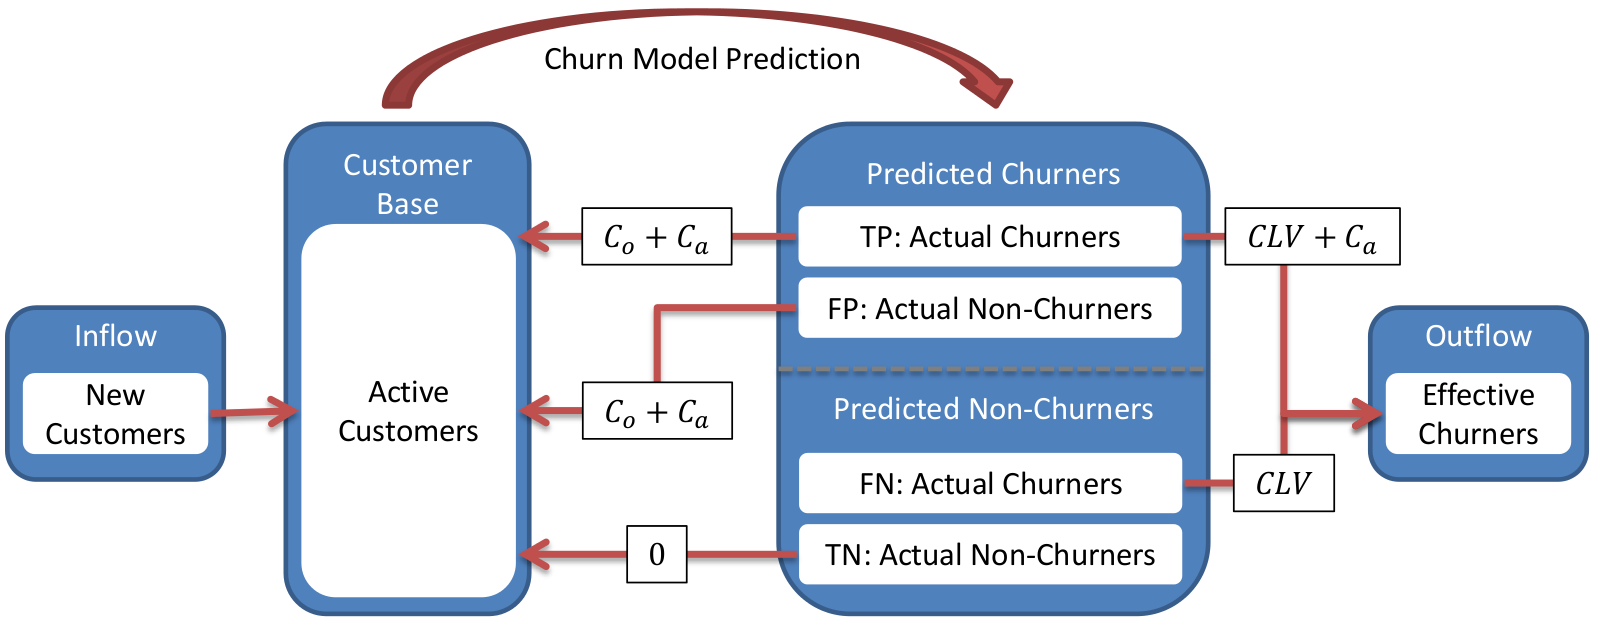
\includegraphics[width=12cm]{ch4_fig2}
  \caption{Financial impact of the different decisions ie. False positives, false negatives, 
  true 	positives and true negatives}
	\label{fig:ch4:2}
\end{figure}

\begin{remark}{Financial analysis of a churn champaing}
When a customer is predicted to be a churner, an offer is made with the objective of avoiding 
the customer defecting. However, if a customer is actually a churner, he may or not accept the 
offer with a probability $\gamma_i$. If the customer accepts the offer, the financial impact is 
equal to the cost of the offer ($C_{o_i}$) plus the administrative cost of contacting the 
customer ($C_a$). On the other hand, if the customer declines the offer, the cost is the 
expected 	income that the clients would otherwise generate, also called customer lifetime value 
($CLV_i$), 	plus $C_a$. Lastly, if the customer is not actually a churner, he will be happy to 
accept the 	offer and the cost will be $C_{o_i}$ plus $C_a$.
	
In the case that the customer is predicted as non-churner, there are two possible outcomes. 
Either the customer is not a churner, then the cost is zero, or the customer is a churner and the 
cost is $CLV_i$. 
\end{remark}

  \begin{table}[htbp]
	  \centering
	  \footnotesize
     \begin{tabular}{c|c|c}
        \multicolumn{3}{c}{}\\
			\multicolumn{1}{c|}{}  & Actual Positive& Actual Negative \\
			\multicolumn{1}{c|}{} & $y_i=1$& $y_i=0$ \\
			\hline
			Predicted Positive 		& $C_{TP_i}=\gamma_iC_{o_i}$ & 
\multirow{2}{*}{$C_{FP_i}=C_{o_i}+C_a$}\\
%       Predicted Positive    & \multirow{ 
% 2}{*}{$C_{TP_i}=\gamma_iC_{o_i}+(1-\gamma_i)(CLV_i+C_a)$} & 
% \multirow{2}{*}{$C_{FP_i}=C_{o_i}+C_a$}\\
			$c_i=1$ & $+(1-\gamma_i)(CLV_i+C_a)$ &\\
			\hline
			Predicted Negative  	& \multirow{ 2}{*}{$C_{FN_i}=CLV_i$} & \multirow{ 
			2}{*}{$C_{TN_i}=0$} \\
			$c_i=0$ & &\\
			%\hline
		\end{tabular}
		\caption{Proposed churn modeling example-dependent cost matrix}
    \label{tab:ch4:1}
  \end{table}

The different costs are sumarized in \tablename{ \ref{tab:ch4:1}}.	Then using the cost 
matrix, and the example-dependent cost-sensitive framework as described in Section 
\ref{sec:2:csmeasures}, an example-dependent cost statistic is calculated as:
\begin{align}
  Cost_i &= y_i(c_i C_{TP_i} + (1-c_i)C_{FN_i})& \nonumber \\
         &  + (1-y_i)(c_i C_{FP_i} + (1-c_i)C_{TN_i})& \nonumber \\
%          &=y_i(c_i (\gamma_iC_{o_i}+(1-\gamma_i)(CLV_i+C_a))& \nonumber \\
%          & + (1-c_i)CLV_i)& \nonumber \\
%          & +  (1-y_i)(c_i (C_{o_i}+C_a) + (1-c_i)(0)) &\nonumber \\
         &= y_i(c_i\left(\gamma_i(C_{o_i}-CLV_i-C_a)-C_{o_i}\right)+CLV_i)&\nonumber \\
         & +c_i(C_{o_i}+C_a),&
	\end{align}
leading to a total cost of:
\begin{equation}
    Cost = \sum_{i=1}^N Cost_i.
\end{equation}
Furthermore, using (\ref{eq:savings}), the savings are calculated as:
\begin{equation}
  Savings = \frac{Cost_l - Cost}{Cost_l},
\end{equation} 
In almost cases the costless class ($Cost_l$) will be the negative class, as typically the 
distribution of a churn dataset is skewed towards the non-churners \citep{Verbeke2012}. Given that 
$Cost_l$ can be expressed as $Cost(f_0)$, or simply $Cost$ with $c_i=0$ $\forall i$:
\begin{equation}
 Cost_l = \sum_{i=1}^{N} y_i CLV_i.
\end{equation}
This is consistent with the notion that if no model is used, the total cost would be the 
sum of the customer lifetime values of the actual churners, which gives the insight 
that the $Savings$ measure is comparing the financial impact of the campaign of using a 
classification model against no using a model at all.


\subsubsection{Customer Lifetime Value}

Lastly, one of the key values to calculate the $Savings$, is the customer lifetime value. Within 
marketing there exists a common misconception between customer profitability and customer lifetime 
value. The two terms are usually used in an interchangeable way, 
creating confusion of what the actual objective of a churn modeling campaign should be. Several 
studies have proposed models providing a unique definition of both terms 
\citep{Neslin2006,Pfeifer2004,Milne1999a,VanRaaij2003}. Customer 
profitability indicates the difference between the income and the cost 
generated by a customer $i$ during a financial period $t$. It is defined as: 
\begin{equation}
	CP_{i,t} = \mu  \cdot s_{i,t},
\end{equation}
where  $s_{i,t}$ refers to the consumption of customer $i$ during time period $t$, and $\mu$ refers 
to the average marginal profit by unit product usage.  

Moreover, we are interested to see what is the expected income that a particular customer will 
generate in the future, in other words, calculating the expected sum of 
discount future earnings \citep{Neslin2006}. Therefore, the $CLV_i$ is defined as:
\begin{equation}
	CLV_i = \sum_{t=1}^T\frac{\mu \cdot s_{i,t}}{(1+r)^t},
\end{equation}
where $r$ is the discount rate, and $T$ the number of time period.
Typically $T$ should be considered large enough since without prior 
knowledge a customer is expected to keep being a customer for the foreseeable future. In practice 
$T$ is set up to be $\infty$ \citep{Glady2009}. Also, for simplicity it can be assumed that 
$s_{i,t+1}=s_{i,t}\cdot (1+g)$ $\forall {i,t}$, which means that there is a constant growth $g$ in 
the customer consumption. Given that, the customer lifetime value can be re-written as
\begin{equation}
 CLV_i = \sum_{t=1}^\infty\frac{ (1+g)^t}{(1+r)^t}\cdot \mu\cdot s_{i,1},
\end{equation}
which in the case of $g<r$, this is a geometric series meaning that it can be expressed as
\begin{equation}
 CLV_i = \frac{\mu\cdot s_{i,1}}{(r-g)}.
\end{equation}


\subsection{Churn Modeling Database}
\label{sec:4:1:data}

For the analysis we used a dataset provided by a TV cable provider. 
The dataset consists of active customers during the first semester of 2014. 	
The total dataset contains 9,410 individual registries, each one with 45 attributes, 
including a churn label indicating whenever a customer is a churner.
This label was created internally in the company, and can be regarded as highly accurate. 
In the dataset only 455 customers are churners, leading to a churn ratio of 4.83\%.
	
\subsubsection{Offer acceptance calculation}

In practice companies have a set of offers to make to a customer as a part of the retention 
campaign, they vary from discounts, to upgrades among others. In the particular case of a TV cable 
provided, the offers include adding a new set of channels, changing the TV receiver to one with new 
technology (ie. high definition, video recording, 4K),  or to offer a discount on the monthly bill.
Unsurprisingly, not all offers apply to all clients. For instance a customer that already has all 
the channels can not be offered a new set of channels. Moreover, an offer usually means an 
additional cost to the company and not all offers have not the same cost or the same impact in 
reducing churn.

Taking into account the cost and the implication of the offers, the problem can be 
resumed in making each customer the offer that will maximize the acceptance rate and more 
important reducing the overall cost. 

\begin{figure}[t!]
  \centering
   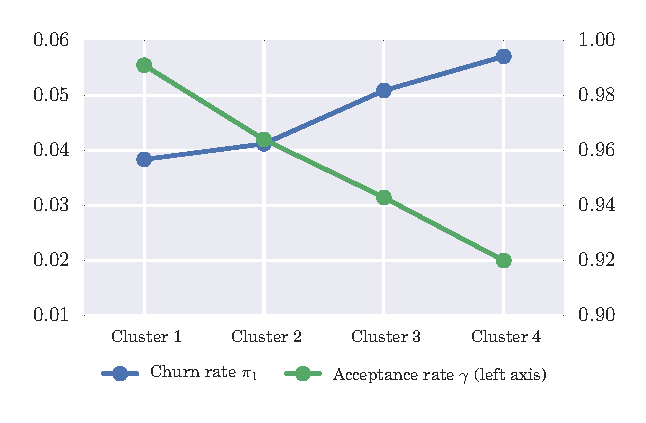
\includegraphics[width=10cm]{ch4_fig3}
  \caption{Acceptance rate ($\gamma$) of the best offer for each customer profile. As expected, 
	the higher the churn rate the lower the acceptance rate, as it is more difficult to make a 
	good offer to a customer which is more likely to defect. }
  \label{fig:ch4:3}
\end{figure}

In order to calculate the acceptance probability $\gamma_i$ a champion-challenger process was made. 
First, the customers were grouped into clusters according to their behavioral and socio-economical 
characteristics. In particular the K-means algorithm was used \citep{Marslan2009}.
Then for a period of two months, randomly selected offers were made to the customers and their 
response was evaluated. Unfortunately, for confidentiality reasons we can not describe the 
different clusters, neither the actual offer made to each customer. Nevertheless, in \figurename{ 
\ref{fig:ch4:3}}, the average churn rate and acceptance rate $\gamma_i$ per cluster is shown. As 
expected, the higher the churn rate the lower the acceptance rate, as it is more difficult to make a 
good offer to a customer which is more likely to defect.


% 	\subsubsection{Database partitioning}
% 	From the initial dataset, three different datasets are extracted: training, validation and 
%   testing. Each one containing 50\%, 25\% and 25\% of the examples, respectively.   
%   Afterwards, with the objective of having a more balanced dataset, ie. same distribution of 
% 	churners and not churners, an under-sampling of the churners is made.     
%   Lastly, we also applied the cost-sensitive re-balancing techniques cost-proportionate 
% 	rejection-sampling \citep{Zadrozny2003} and cost-proportionate over-sampling \citep{Elkan2001}, 
% 	described in cost-sensitive classification Section.
% 	\tablename{ \ref{table_trainandtest}}, summarizes the different datasets, where $N$, $\pi_1$ 
% and $C_0$ represents the number of customers, the percentage of churners and the total losses if no 
% model is used, respectively. Moreover, in \figurename{ \ref{fig:ch5:4}}, a comparison of the 
% churn rate 
% and the average unitary cost ($C_u=C_0 / N$) of each dataset with respect of the Total set is shown.
% It is observed that the cost-sensitive sampling procedures have an average unitary cost much higher 
% than the other sets, also showing why a simple under-sampling procedure of the dataset does not 
% take into account the costs.
% 
%   \begin{table}[t!]
%     \caption{Description of datasets}
%     \label{table_trainandtest}
%     \centering
%     \begin{tabular}{l c c c } %sum 7.7
% 		\\ \hline
% 		Set&	$N$ &	$\pi_1$ & $C_0$ \\
% 		\hline
% 		Total&9,410&.0483&580,884\\
% 		Training ($t$)&3,758&.0505&244,542\\
% 		Validation&2,824&.0477&174,171\\
% 		Testing&2,825&.0442&162,171\\
% 		Under-sampling ($u$)&374&.5080&244,542\\
% 		CS Rejection-sampling ($r$)&428&.4135&431,428\\
% 		CS Over-sampling ($o$)&5,767&.03124&2,350,285\\
% 	  \hline
% 	  \end{tabular}
%   \end{table}
% 
% 	\begin{figure}[t!]
% 	  \centering
%     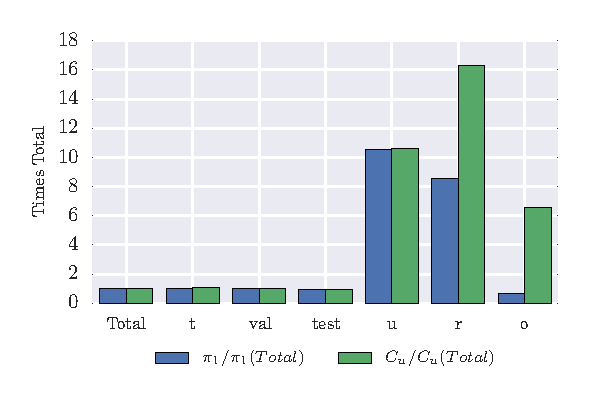
\includegraphics{ch5_fig4}
% 	  \caption{Comparison of the distribution of the churn rate and the average unitary cost 
% 	  ($C_u=C_0 / N$) of each dataset with respect to the Total set.
% It is observed that the cost-sensitive sampling procedures have an average unitary cost much higher 
% than the other sets, also showing why a simple under-sampling procedure of the dataset does not 
% take into account the costs.}
% 	  \label{fig:ch5:4}
% 	\end{figure}


\section{Direct marketing}
\label{sec:4:directmarketing}

In direct marketing the objective is to classify those customers who are more likely to have a 
certain response to a marketing campaign \citep{Ngai2009}. We used a direct marketing dataset 
\citep{Moro2011} available on the UCI machine learning repository \citep{UCI2013}. The dataset 
contains 45,000 clients of a Portuguese bank who were contacted by phone between March 2008 and 
October 2010 and received an offer to open a long-term deposit account with attractive interest 
rates.  The dataset contains features such as age, job, marital status, education, average yearly 
balance and current loan status and the label indicating whether or not the client accepted 
the offer.

This problem is example-dependent cost sensitive, since there are different costs of false 
positives and false negatives. Specifically, in direct marketing, false positives have the cost 
of contacting the client, and false negatives have the cost due to the loss of income by failing 
to contact a client that otherwise would have opened a long-term deposit. 
  
\begin{table}[!t]
  \centering
  \footnotesize
  \begin{tabular}{c|c|c}
    \multicolumn{1}{c|}{}  & Actual Positive& Actual Negative \\
    \multicolumn{1}{c|}{} & $y_i=1$& $y_i=0$ \\
    \hline
    Predicted Positive 		& \multirow{ 2}{*}{$C_{TP_i}=C_a$} & \multirow{ 2}{*}{$C_{FP_i}=C_a$} 
    \\
    $c_i=1$ & &\\
    \hline
    Predicted Negative  	& \multirow{ 2}{*}{$C_{FN_i}=Int_i$} & \multirow{ 2}{*}{$C_{TN_i}=0$} 
    \\
    $c_i=0$ & &\\
    %\hline
  \end{tabular}
  \caption{Direct marketing example-dependent cost matrix}
  \label{tab:4:d_mat}
\end{table}
		
We used the direct marketing example-dependent cost matrix proposed in \citep{CorreaBahnsen2014}. 
The cost matrix is shown in \mbox{\tablename{ \ref{tab:4:d_mat}}}, where $C_a$ is the 
administrative cost of contacting the client, as is credit card fraud,  and $Int_i$ is the expected 
income when a client opens a long-term deposit. This last term is defined as the long-term deposit 
amount times the interest rate spread.
 
In order to estimate $Int_i$, first the long-term deposit amount is assumed to be a 20\% of the 
average yearly balance, and lastly, the interest rate spread is estimated to be 2.463333\%,	which 
is the average between 2008 and 2010 of the retail banking sector in Portugal as reported by the 
Portuguese central bank. Given that, the $Int_i$ is equal to $\left( balance * 20\% \right) * 
2.463333\%$.
		
% Subsequently, the dataset is split in training, under-sampling, validation and test. Relevant 
% information of the datasets is shown in \tablename{ \ref{table_fraud_trainandtest_marketing}}.
% \footnotetext{Interest rate spread is the difference between the effective lending rate and the 
% cost of funds.}
%  
% 	\begin{table}[!t]
% 	\caption{Description of datasets of the direct marketing dataset}
% 	\label{table_fraud_trainandtest_marketing}
% 	\centering
% 	\begin{tabular}{|c|c|c|c|} %sum 7.7
% 		\hline
% 		Database&	No Trx&	Accept&$Int$\\
% 		\hline	
% 		Total& 47,562&	12.56\%&	394,211\\
% 		\hline
% 		Train& 19,119&12.64\%&	156,676\\   
% 		Undersampled&4,819&50.17\%&42,443   \\
% 		\hline
% 		Validation& 11,809&12.78\%&97,498   \\
% 		Test& 11,815&12.23\%&97,594   \\
% 		\hline
% 	\end{tabular}
% 	\end{table}
% 	
